
\documentclass[12pt]{article}
\usepackage[margin = 1in]{geometry}
\usepackage[dvipsnames]{xcolor}
\usepackage{tabularx}
\usepackage{graphicx}
\usepackage{enumitem}
\usepackage{hyperref}
% \usepackage{fancyhdr}
\usepackage[margin = 0cm]{caption}
\usepackage{wrapfig}
\usepackage{amsmath}
\usepackage{amssymb}
\usepackage{natbib}
\setlength{\bibsep}{0pt}
\hypersetup{ % all blue links
	colorlinks		= true,
	urlcolor 		= blue,
	linkcolor 		= blue,
	citecolor 		= blue
}
\setcitestyle{aysep={}, yysep={,}}
\newcommand{\aj}{AJ}
\newcommand{\aap}{A\&A}
\newcommand{\aapr}{A\&ARv}
\newcommand{\apj}{ApJ}
\newcommand{\apjl}{ApJL}
\newcommand{\apjs}{ApJS}
\newcommand{\apss}{Ap\&SS}
\newcommand{\araa}{ARA\&A}
\newcommand{\baas}{BAAS}
\newcommand{\fcp}{Fundamentals Cosmic Phys.}
\newcommand{\mnras}{MNRAS}
\newcommand{\nat}{Nature}
\newcommand{\pasa}{PASA}
\newcommand{\pasp}{PASP}
\newcommand{\ddfrac}[2]{\frac{\displaystyle{#1}}{\displaystyle{#2}}}
\newcommand{\msun}{\ensuremath{\text{M}_\odot}}
\newcommand{\scinote}[2]{\ensuremath{#1\times10^{#2}}}
\providecommand{\noopsort}[1]{}

\begin{document}

\begin{center}
\textbf{The Impact of the IMF on Chemical Evolution Models}
\par\null\par
James W. Johnson
\par\null\par
\rule[0.7\baselineskip]{0.5\textwidth}{0.4pt}
\end{center}

\par\noindent
\textbf{Population-Averaged Yields from Massive Stars}
\par\noindent
\begin{wrapfigure}{r}{0.5\textwidth}
\centering
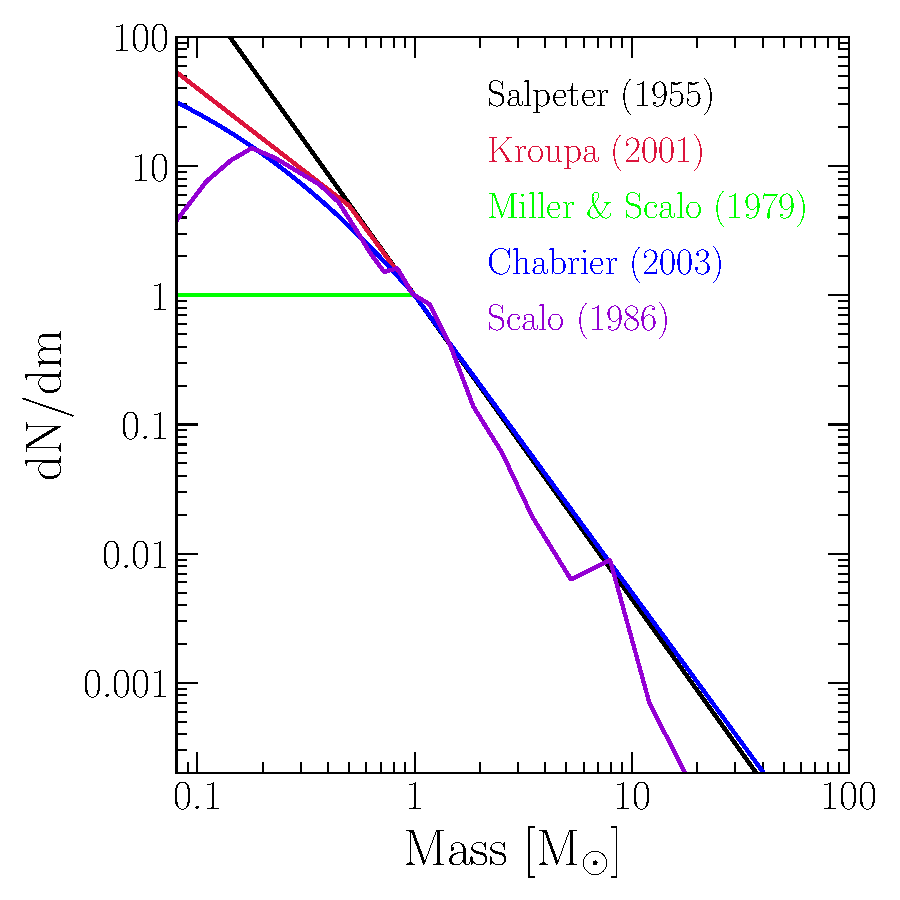
\includegraphics[scale = 0.5]{imfs.pdf}
\caption{
A compilation of popular choices of IMF in the literature:
\citet[][black]{Salpeter1955},~\citet[][red]{Kroupa2001},
\citet[][green]{Miller1979},~\citet[][blue]{Chabrier2003}, and
\citet[][purple]{Scalo1986}, all normalized to a value of 1 at~$M = 1$~\msun.
}
\label{fig:imfs}
\end{wrapfigure}
The chemical enrichment histories of galaxies are, to first order, determined
by population-averaged yields from stellar populations, which is in turn
sensitive to the choice of initial mass function (IMF).
Fig.~\ref{fig:imfs} illustrates a handful of IMFs that are common in the
literature.
While the others are presented as analytic functional forms, the
\citet{Scalo1986} IMF is computed from tabulated data, which I'm here
interpolating between in~$\log_{10} M$.
\par
The~\citet{Scalo1986} IMF is used by~\citet*{Minchev2013} and
\citet{Spitoni2019}, both of whom present chemical evolution models of the
Galactic disk which assume no significant mass loading in outflows.
The defining feature of~\citet{Scalo1986} compared to other IMFs is that it is
noticeably steeper at the high mass end.
However, this IMF is expected to be deficient in massive stars as
\citet{Scalo1986} accounted for neither the time these stars remain obscured by
their parent clouds nor the largest OB associations (see discussion
in~\S~2.2.2 of~\citealt*{Parravano2011}).
\par
I next compute IMF-averaged yields of various elements based on the
\citet{Sukhbold2016} massive star yield tables with the W18 explosion engine
according to
\begin{equation}
y_\text{x}^\text{CC} = \ddfrac{
	\int_{l_\text{cc}}^u (E(m)m_x + w_x - Z_\text{x,prog}(m - m_\text{rem}(m)))
	\frac{dN}{dm}dm
}{
	\int_l^u m\frac{dN}{dm}dm
},
\label{eq:y_x_cc}
\end{equation}
where $l_\text{cc} = 8$~\msun~is the assumed lower mass limit of a core
collapse SN progenitor and~$l = 0.08$~\msun~and~$u = 120$~\msun~are the lower
and upper mass limits of star formation.
$E(m)$ is the fraction of stars of initial mass~$m$ that explode as a CCSN,
$w_x$ is the wind yield, and~$Z_\text{x,prog}(m - m_\text{rem})$ converts from
a gross yield to a net yield of some element x.
$E(m)$ is included~\textit{a priori} in the W18 explosion engine as the stars
which fail to explode are assigned an explosive yield of~$m_x = 0$.
To quantify the impact of the IMF, I first compute values
of~$y_\text{x}^\text{CC}$ assuming the~\citet{Kroupa2001} IMF, then compute
the factor by which it changes for a different IMF.
I show results for 30 elements in Fig.~\ref{fig:imfs}.

\begin{figure*}
\centering
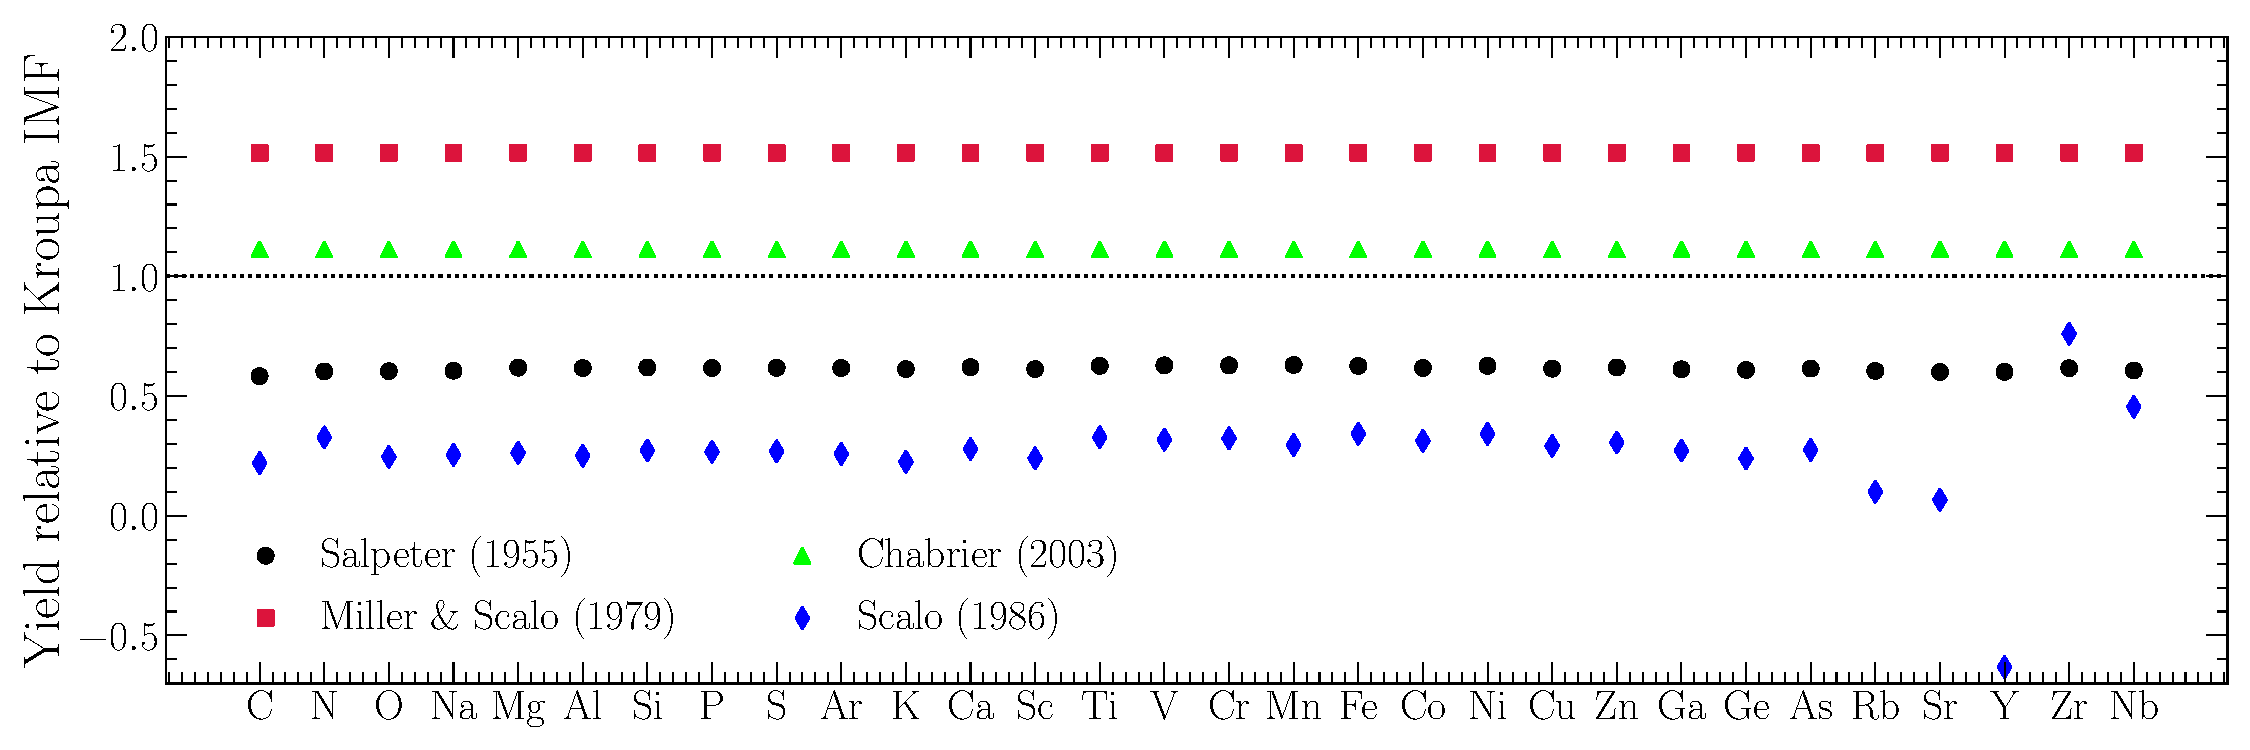
\includegraphics[scale = 0.42]{yields_relative_to_kroupa.pdf}
\caption{
The impact of the IMF on population-averaged massive star elemental yields.
For any given IMF as indicated by the legend, the yield is given by
equation~\ref{eq:y_x_cc} and normalized by the value computed for
the~\citet{Kroupa2001} IMF.
}
\label{fig:yields}
\end{figure*}

For alpha and iron-peak elements, the choice of IMF affects the
population-averaged yield at the factor of~$\sim$5 level (i.e., ratios of
$\sim$0.3 to~$\sim$1.5).
In the case of the~\citet{Salpeter1955},~\citet{Miller1979},
and~\citet{Chabrier2003} IMFs, this sensitivity arises due to different
frequencies of low-mass stars.
Of these three,~\citet{Salpeter1955} has the most low-mass stars -- or
conversely the fewest high-mass stars -- and consequently the lowest
population-averaged yields.
In the case of the~\citet{Scalo1986} IMF, the steeper slope at the high-mass
end also contributes to lowering the overall yield.
For s-process elements, however, the~\citet{Scalo1986} IMF does not affect
population-averaged yields with an approximately uniform multiplicative factor.
This difference arises due to net versus gross yields; in a version of this
figure computed with gross yields (i.e., simply setting $Z_\text{x,prog} = 0$),
the yields of s-process elements predicted by the~\citet{Scalo1986} IMF were
indeed~$\sim$30\% of the yields computed with the~\citet{Kroupa2001} IMF.
Inspection of the W18 yield tables from~\citet{Sukhbold2016} indicates that the
highest mass stars have the largest yields of Sr and Y, and this contribution
is down-weighted by the steep~\citet{Scalo1986} IMF, making the net yield
negative in the case of Y.
\par\null\par\noindent
\textbf{One-Zone Models: Alpha and Iron-peak Elements}
\par\noindent
Before exploring chemical evolution models with different IMFs, and
consequently different population-averaged elemental yields, a choice must be
made as to how to handle the Type Ia SN yields of Fe~$y_\text{Fe}^\text{Ia}$
Here I simply set~$y_\text{Fe}^\text{Ia}$ to a value which implies a solar
equilibrium [O/Fe] abundance ratio for a constant SFH.
The equililbrium abundance ratio can be expressed as:
\begin{subequations}\begin{align}
[\text{O/Fe}]_\text{eq} &=
\log_{10}\left(\frac{Z_\text{O,eq}}{Z_\text{Fe,eq}}\right) -
\log_{10}\left(\frac{Z_{\text{O},\odot}}{Z_{\text{Fe},\odot}}\right)
\\
&= \log_{10}\left(\frac{y_\text{O}^\text{CC}}{y_\text{Fe}^\text{CC} +
y_\text{Fe}^\text{Ia}(\langle\dot{M}_\star\rangle_\text{Ia} / \dot{M}_\star)}
\right) -
\log_{10}\left(\frac{Z_{\text{O},\odot}}{Z_{\text{Fe},\odot}}\right),
\end{align}\end{subequations}
where~$\langle\dot{M}_\star\rangle_\text{Ia}$ is the time-integrated SFH
weighted by the SN Ia DTD and~$\dot{M}_\star$ is the present-day SFR.
The ratio between these quantities accounts for differences in the equilibrium
Fe abundance due to differently shaped SFHs.
For further details, see discussion in~\citet*{Weinberg2017}.
\par
Rearranging this equation to solve for~$y_\text{Fe}^\text{Ia}$ yields the
following expression:
\begin{equation}
y_\text{Fe}^\text{Ia} =
\frac{\dot{M}_\star}{\langle\dot{M}_\star\rangle_\text{Ia}}
\left(
y_\text{O}^\text{CC} 10^{-[\text{O/Fe}]_\text{eq}}
\left(\frac{Z_{\text{Fe},\odot}}{Z_{\text{O},\odot}}\right) -
y_\text{Fe}^\text{CC}
\right).
\end{equation}
If the SFH is constant, then the factor~$\dot{M}_\star /
\langle\dot{M}_\star\rangle_\text{Ia} \approx 1$ for any steeply declining
DTD.
Assuming~$\sim$solar equilibrium abundances (i.e., [O/Fe]$_\text{eq}$ = 0)
then yields
\begin{equation}
y_\text{Fe}^\text{Ia} = y_\text{O}^\text{CC}
\left(\frac{Z_{\text{Fe},\odot}}{Z_{\text{O},\odot}}\right) -
y_\text{Fe}^\text{CC}.
\label{eq:y_fe_ia}
\end{equation}
The SN yields computed from equations~\ref{eq:y_x_cc} and~\ref{eq:y_fe_ia} for
each IMF are given in Table~\ref{tab:yields}.

{%
\renewcommand{\arraystretch}{1.2}
\begin{table*}
\caption{
The values of~$y_\text{O}^\text{CC}$ and~$y_\text{Fe}^\text{CC}$ computed from
equation~\ref{eq:y_x_cc} and~$y_\text{Fe}^\text{Ia}$ computed from
equation~\ref{eq:y_fe_ia} for the various IMFs considered here.
}
\begin{tabularx}{\textwidth}{l @{\extracolsep{\fill}} l l l}
\hline
IMF & $y_\text{O}^\text{CC}$ & $y_\text{Fe}^\text{CC}$ & $y_\text{Fe}^\text{Ia}$
\\
\hline
\citet{Kroupa2001} & 0.00571 & \scinote{4.72}{-4} & \scinote{8.15}{-4}
\\
\citet{Salpeter1955} & 0.00345 & \scinote{2.96}{-4} & \scinote{4.82}{-4}
\\
\citet{Miller1979} & 0.00865 & \scinote{7.16}{-4} & 0.00124
\\
\citet{Chabrier2003} & 0.00635 & \scinote{5.25}{-4} & \scinote{9.06}{-4}
\\
\citet{Scalo1986} & 0.00140 & \scinote{1.61}{-4} & \scinote{1.55}{-4}
\\
\hline
\end{tabularx}
\label{tab:yields}
\end{table*}
}

\begin{figure*}
\centering
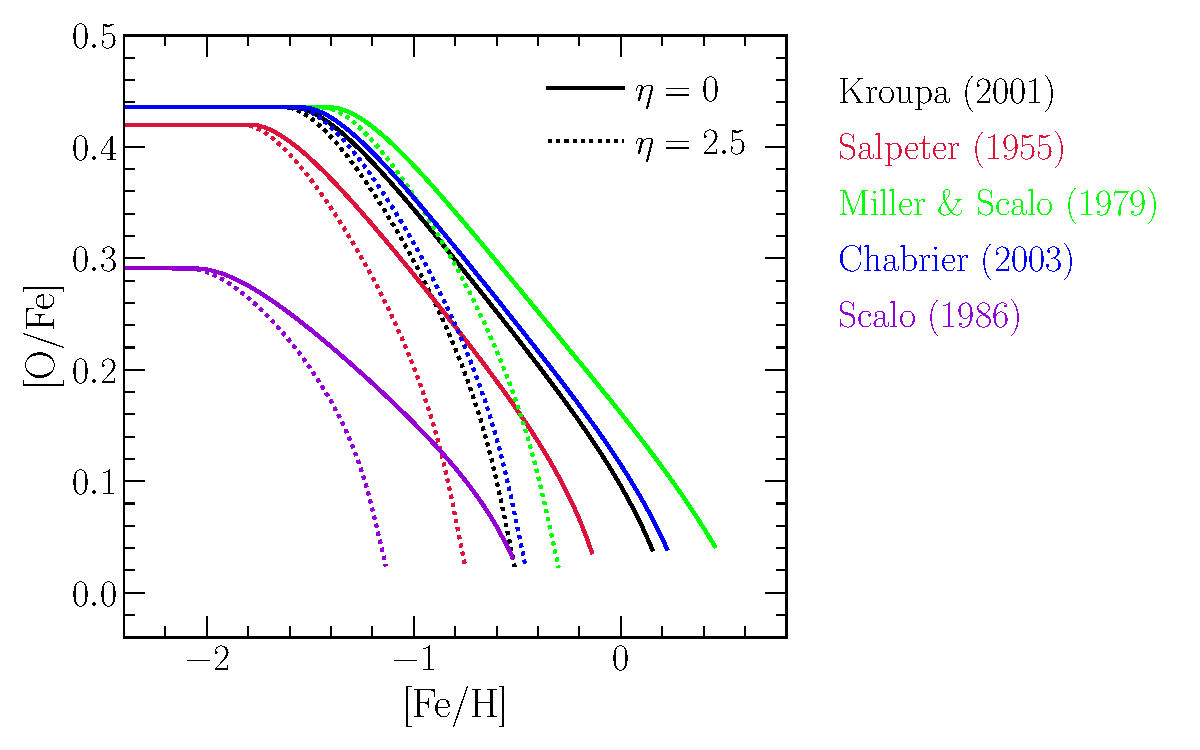
\includegraphics[scale = 0.6]{onezone_different_imfs.pdf}
\caption{
One-zone GCE models computed assuming a constant SFH and the yields given in
Table~\ref{tab:yields} for each IMF noted in the legend.
Solid lines show the evolution predicted with no mass loading in outflows
(i.e.,~$\eta = 0$), while dotted lines show the predictions with~$\eta = 2.5$.
}
\label{fig:onezone}
\end{figure*}

The predicted evolutionary tracks in the gas-phase for each of these IMFs with
yields adjusted accordingly are shown in Fig.~\ref{fig:onezone}.
In all cases, the late-time abundance ratios with~$\eta > 0$ are below the
abundances predicted with~$\eta = 0$, a direct consequence of the lowered
equilibrium ratios due to the strong sink term of mass loading (see discussion
in~\citealt{Weinberg2017}).
The position of the plateau is largely determined by the slope of the IMF at
the high-mass end.
The~\citet{Kroupa2001},~\citet{Miller1979}, and~\citet{Chabrier2003} each have
a slope of~$-2.3$ and a plateau at [O/Fe]~$\approx +0.44$.
The~\citet{Salpeter1955}, with a slope of~$-2.35$, has a slightly lower plateau
at [O/Fe]~$\approx +0.42$.
The~\citet{Scalo1986}, the steepest of them all, has the lowest plateau at
[O/Fe]~$\approx +0.29$.
Although yields of alpha and iron-peak elements are affected similarly by the
choice of IMF, 0.1 dex corresponds only to a difference of~$\sim$26\%, so the
small fluctuations in the inferred yield relative to the~\citet{Kroupa2001} IMF
in Fig.~\ref{fig:yields} are more apparent on the y-axis of
Fig.~\ref{fig:onezone}.
Higher plateau heights with the~\citet{Scalo1986} IMF are achievable with
different yield sets; for example,~\citet{Spitoni2019} use massive star yields
from~\citet{Woosley1995}, which produces a plateau at [O/Fe]~$\approx +0.53$.
\par
The left-right separation of tracks contains information on the abundance of
low-mass stars.
Of the~\citet{Kroupa2001},~\citet{Miller1979},~\citet{Chabrier2003} IMFs at the
same plateau in [O/Fe], the~\citet{Miller1979} form has the fewest low-mass
stars, and the highest [Fe/H] track.
Conversely,~\citet{Kroupa2001} has the most low-mass stars and the lowest
[Fe/H] track of these three IMFs.
\par
Although the~\citet{Kroupa2001} and~\citet{Chabrier2003} are arguably the most
realistic of these IMFs, this comparison clearly demonstrates the degree of
model dependence when a different IMF is adopted.
In particular,~\citet{Spitoni2020} adopt the~\citet{Scalo1986} IMF and conduct
an MCMC fit of the two-infall model to the APOKASC sample presented by
\citet{SilvaAguirre2018}.
With a different choice of IMF, they would likely infer different evolutionary
parameters for the two infall events due to this model dependence.

% \newpage
\bibliographystyle{mnras}
\bibliography{yields-onezone}

\end{document}

